\subsection{Task overheads}
Having discovered that a significant portion of the time spent running small tasks is in deserialization, we further measured the time it took individual components of deserialization to complete. What we found is that in order to reduce the amount of duplicate data transferred, Spark 1.1.0 made the bytes containing the RDD to use and the function to run on it a broadcast variable. Since an executor can simultaneously process many tasks, this change means the bytes will only be sent once. The first task that uses the information will pull it from the master, and cache the result with the executor for later tasks. In the Spark Streaming context however, this means for every stage, some task on every executor requires a round trip to the driver to fetch the broadcast variable, increasing the latency. Furthermore, as the batch interval shrinks, new RDDs are created more often, but the function to operate on them does not change. The executor should be able to cache it for a longer period of time than only for the current stage. [talk about results here?]

Another interesting discovery regarding the deserialization time is that after the information regarding the new files and JARs needed by the task is deserialized, the executor calls a function to update the dependencies. But in this function, the original implementation creates a new Hadoop configuration object every time, despite the fact that it is rarely used. Since creating a new Hadoop configuration is costly in CPU cycles, we made the instantiation of the object lazy, and saw an order of magnitude improvement in the execution time of that function.


\subsection{Scheduling scalability}

\begin{figure}[h!]
  \begin{center}
    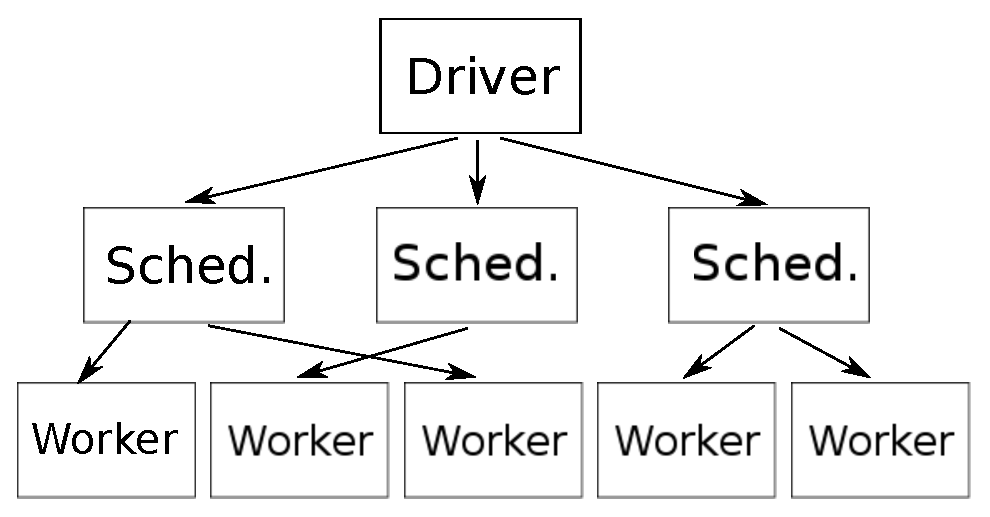
\includegraphics[scale=0.45]{scheduler_architecture.eps}
  \end{center}
  \caption{Proposed scheduler architecture.}
  \label{fig:schedarch}
\end{figure}

To enable a higher scheduling rate of tasks by Spark Streaming we propose 1) scheduling all tasks per worker in bulk and 2) physically decoupling the scheduling (Scheduler) of tasks from the generation (Driver).
First, at each scheduling stage, instead of sending multiple tasks for each node separately, we coalesce them into the same message. This reduces the serialization and networking overheads that result from sending many small messages.
Secondly, as the task generation rate surpasses the scheduling rate, the driver elastically spawns schedulers in remote physical nodes. Thereafter, tasks are forwarded, according to some policy, to these newly spawned schedulers for scheduling (see Fig. \ref{fig:schedarch}). 

We have implemented this solution in Spark Streaming.
